

% %% comienzo de la parte de anexos
% \appendixpart

% %% contenido del primer anexo
% \appendix{Experimental results charts}

% \section{Base benchmark}

% \begin{figure}[!ht]
%     \centering
%     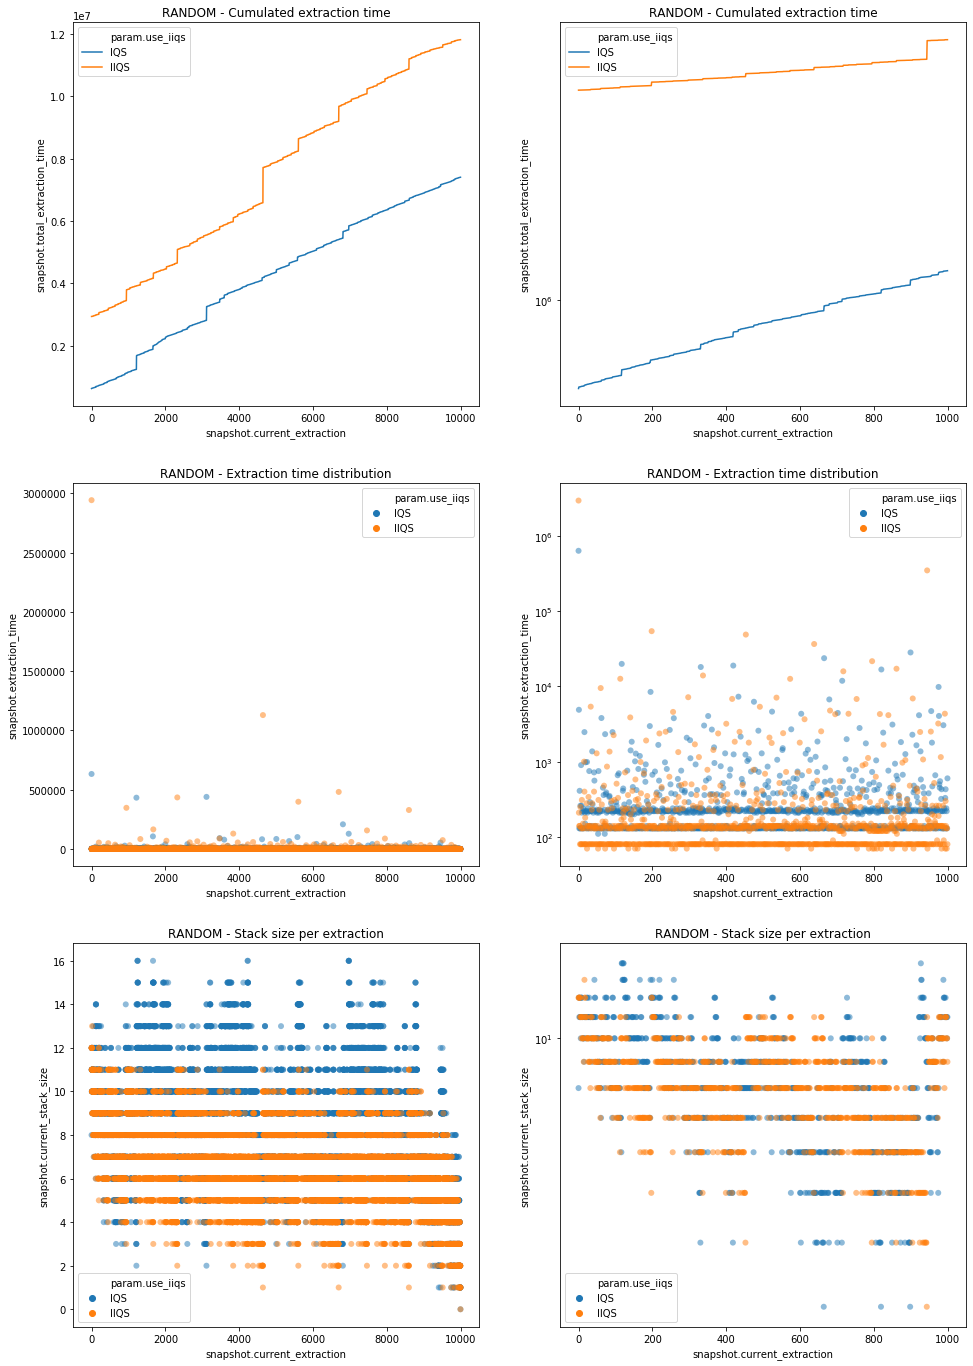
\includegraphics[width=0.8\textwidth]{./fragments/04_experimental_execution/images/01_basebenchmark_01_random_case.png}
%     %\caption{Benchmark for random case. IQS and IIQS executions are shown on the first and second columns respectively.}
%     \caption{Benchmark for random case for sequences with $1\times10^4$ elements. Both IQS and IIQS executions are shown on the same chart. First column represents all extractions using a linear scale. Second column depicts a logarithmic scale and shows the first $1\times10^3$ extractions.}
%     \label{FIG:BENCHMARK_01_RANDOM_CASE}
% \end{figure}

% \section{La segunda sección del primer anexo}
% Aquí va el texto de la segunda sección del primer anexo...

% \subsection{La primera subsección de la segunda sección del primer anexo}


% %% contenido del segundo anexo
% \appendix{El segundo Anexo}
% Aquí va el texto del segundo anexo...

% \section{La primera sección del segundo anexo}
% Aquí va el texto de la primera sección del segundo anexo...